\documentclass{book}
\usepackage{amsmath,amssymb}
\usepackage{lipsum}
\usepackage{tikz}
\usepackage{hyperref}
\begin{document}
\tableofcontents
\chapter{Chapter 1}\label{ch:1}
\section{Section 1.1}\label{sec:1-1}
See Chapter~\ref{ch:1} and Section~\ref{sec:1-1}.
\lipsum[7-9]
\begin{equation}\label{eq:1-1} \int_0^{1} x^{1}\,dx = \frac{1^{2}}{2}\end{equation}
\section{Section 1.2}\label{sec:1-2}
See Chapter~\ref{ch:1} and Section~\ref{sec:1-2}.
\lipsum[8-10]
\begin{equation}\label{eq:1-2} \int_0^{2} x^{1}\,dx = \frac{2^{2}}{2}\end{equation}
\section{Section 1.3}\label{sec:1-3}
See Chapter~\ref{ch:1} and Section~\ref{sec:1-3}.
\lipsum[9-11]
\begin{equation}\label{eq:1-3} \int_0^{3} x^{1}\,dx = \frac{3^{2}}{2}\end{equation}
\section{Section 1.4}\label{sec:1-4}
See Chapter~\ref{ch:1} and Section~\ref{sec:1-4}.
\lipsum[10-12]
\begin{equation}\label{eq:1-4} \int_0^{4} x^{1}\,dx = \frac{4^{2}}{2}\end{equation}
\section{Section 1.5}\label{sec:1-5}
See Chapter~\ref{ch:1} and Section~\ref{sec:1-5}.
\lipsum[11-13]
\begin{equation}\label{eq:1-5} \int_0^{5} x^{1}\,dx = \frac{5^{2}}{2}\end{equation}
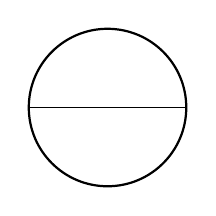
\begin{tikzpicture}\draw[thick] (0,0) circle (1); \draw (-1,0)--(1,0);\end{tikzpicture}
\chapter{Chapter 2}\label{ch:2}
\section{Section 2.1}\label{sec:2-1}
See Chapter~\ref{ch:1} and Section~\ref{sec:2-1}.
\lipsum[12-14]
\begin{equation}\label{eq:2-1} \int_0^{1} x^{2}\,dx = \frac{1^{3}}{3}\end{equation}
\section{Section 2.2}\label{sec:2-2}
See Chapter~\ref{ch:1} and Section~\ref{sec:2-2}.
\lipsum[13-15]
\begin{equation}\label{eq:2-2} \int_0^{2} x^{2}\,dx = \frac{2^{3}}{3}\end{equation}
\section{Section 2.3}\label{sec:2-3}
See Chapter~\ref{ch:1} and Section~\ref{sec:2-3}.
\lipsum[14-16]
\begin{equation}\label{eq:2-3} \int_0^{3} x^{2}\,dx = \frac{3^{3}}{3}\end{equation}
\section{Section 2.4}\label{sec:2-4}
See Chapter~\ref{ch:1} and Section~\ref{sec:2-4}.
\lipsum[15-17]
\begin{equation}\label{eq:2-4} \int_0^{4} x^{2}\,dx = \frac{4^{3}}{3}\end{equation}
\section{Section 2.5}\label{sec:2-5}
See Chapter~\ref{ch:1} and Section~\ref{sec:2-5}.
\lipsum[16-18]
\begin{equation}\label{eq:2-5} \int_0^{5} x^{2}\,dx = \frac{5^{3}}{3}\end{equation}
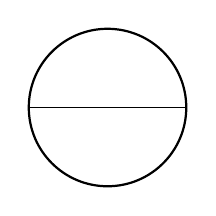
\begin{tikzpicture}\draw[thick] (0,0) circle (1); \draw (-1,0)--(1,0);\end{tikzpicture}
\chapter{Chapter 3}\label{ch:3}
\section{Section 3.1}\label{sec:3-1}
See Chapter~\ref{ch:2} and Section~\ref{sec:3-1}.
\lipsum[17-19]
\begin{equation}\label{eq:3-1} \int_0^{1} x^{3}\,dx = \frac{1^{4}}{4}\end{equation}
\section{Section 3.2}\label{sec:3-2}
See Chapter~\ref{ch:2} and Section~\ref{sec:3-2}.
\lipsum[18-20]
\begin{equation}\label{eq:3-2} \int_0^{2} x^{3}\,dx = \frac{2^{4}}{4}\end{equation}
\section{Section 3.3}\label{sec:3-3}
See Chapter~\ref{ch:2} and Section~\ref{sec:3-3}.
\lipsum[19-21]
\begin{equation}\label{eq:3-3} \int_0^{3} x^{3}\,dx = \frac{3^{4}}{4}\end{equation}
\section{Section 3.4}\label{sec:3-4}
See Chapter~\ref{ch:2} and Section~\ref{sec:3-4}.
\lipsum[20-22]
\begin{equation}\label{eq:3-4} \int_0^{4} x^{3}\,dx = \frac{4^{4}}{4}\end{equation}
\section{Section 3.5}\label{sec:3-5}
See Chapter~\ref{ch:2} and Section~\ref{sec:3-5}.
\lipsum[21-23]
\begin{equation}\label{eq:3-5} \int_0^{5} x^{3}\,dx = \frac{5^{4}}{4}\end{equation}
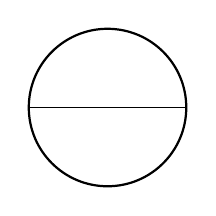
\begin{tikzpicture}\draw[thick] (0,0) circle (1); \draw (-1,0)--(1,0);\end{tikzpicture}
\chapter{Chapter 4}\label{ch:4}
\section{Section 4.1}\label{sec:4-1}
See Chapter~\ref{ch:3} and Section~\ref{sec:4-1}.
\lipsum[22-24]
\begin{equation}\label{eq:4-1} \int_0^{1} x^{4}\,dx = \frac{1^{5}}{5}\end{equation}
\section{Section 4.2}\label{sec:4-2}
See Chapter~\ref{ch:3} and Section~\ref{sec:4-2}.
\lipsum[23-25]
\begin{equation}\label{eq:4-2} \int_0^{2} x^{4}\,dx = \frac{2^{5}}{5}\end{equation}
\section{Section 4.3}\label{sec:4-3}
See Chapter~\ref{ch:3} and Section~\ref{sec:4-3}.
\lipsum[24-26]
\begin{equation}\label{eq:4-3} \int_0^{3} x^{4}\,dx = \frac{3^{5}}{5}\end{equation}
\section{Section 4.4}\label{sec:4-4}
See Chapter~\ref{ch:3} and Section~\ref{sec:4-4}.
\lipsum[25-27]
\begin{equation}\label{eq:4-4} \int_0^{4} x^{4}\,dx = \frac{4^{5}}{5}\end{equation}
\section{Section 4.5}\label{sec:4-5}
See Chapter~\ref{ch:3} and Section~\ref{sec:4-5}.
\lipsum[26-28]
\begin{equation}\label{eq:4-5} \int_0^{5} x^{4}\,dx = \frac{5^{5}}{5}\end{equation}
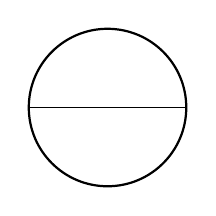
\begin{tikzpicture}\draw[thick] (0,0) circle (1); \draw (-1,0)--(1,0);\end{tikzpicture}
\chapter{Chapter 5}\label{ch:5}
\section{Section 5.1}\label{sec:5-1}
See Chapter~\ref{ch:4} and Section~\ref{sec:5-1}.
\lipsum[27-29]
\begin{equation}\label{eq:5-1} \int_0^{1} x^{5}\,dx = \frac{1^{6}}{6}\end{equation}
\section{Section 5.2}\label{sec:5-2}
See Chapter~\ref{ch:4} and Section~\ref{sec:5-2}.
\lipsum[28-30]
\begin{equation}\label{eq:5-2} \int_0^{2} x^{5}\,dx = \frac{2^{6}}{6}\end{equation}
\section{Section 5.3}\label{sec:5-3}
See Chapter~\ref{ch:4} and Section~\ref{sec:5-3}.
\lipsum[29-31]
\begin{equation}\label{eq:5-3} \int_0^{3} x^{5}\,dx = \frac{3^{6}}{6}\end{equation}
\section{Section 5.4}\label{sec:5-4}
See Chapter~\ref{ch:4} and Section~\ref{sec:5-4}.
\lipsum[30-32]
\begin{equation}\label{eq:5-4} \int_0^{4} x^{5}\,dx = \frac{4^{6}}{6}\end{equation}
\section{Section 5.5}\label{sec:5-5}
See Chapter~\ref{ch:4} and Section~\ref{sec:5-5}.
\lipsum[31-33]
\begin{equation}\label{eq:5-5} \int_0^{5} x^{5}\,dx = \frac{5^{6}}{6}\end{equation}
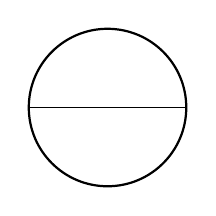
\begin{tikzpicture}\draw[thick] (0,0) circle (1); \draw (-1,0)--(1,0);\end{tikzpicture}
\chapter{Chapter 6}\label{ch:6}
\section{Section 6.1}\label{sec:6-1}
See Chapter~\ref{ch:5} and Section~\ref{sec:6-1}.
\lipsum[32-34]
\begin{equation}\label{eq:6-1} \int_0^{1} x^{6}\,dx = \frac{1^{7}}{7}\end{equation}
\section{Section 6.2}\label{sec:6-2}
See Chapter~\ref{ch:5} and Section~\ref{sec:6-2}.
\lipsum[33-35]
\begin{equation}\label{eq:6-2} \int_0^{2} x^{6}\,dx = \frac{2^{7}}{7}\end{equation}
\section{Section 6.3}\label{sec:6-3}
See Chapter~\ref{ch:5} and Section~\ref{sec:6-3}.
\lipsum[34-36]
\begin{equation}\label{eq:6-3} \int_0^{3} x^{6}\,dx = \frac{3^{7}}{7}\end{equation}
\section{Section 6.4}\label{sec:6-4}
See Chapter~\ref{ch:5} and Section~\ref{sec:6-4}.
\lipsum[35-37]
\begin{equation}\label{eq:6-4} \int_0^{4} x^{6}\,dx = \frac{4^{7}}{7}\end{equation}
\section{Section 6.5}\label{sec:6-5}
See Chapter~\ref{ch:5} and Section~\ref{sec:6-5}.
\lipsum[36-38]
\begin{equation}\label{eq:6-5} \int_0^{5} x^{6}\,dx = \frac{5^{7}}{7}\end{equation}
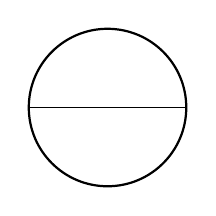
\begin{tikzpicture}\draw[thick] (0,0) circle (1); \draw (-1,0)--(1,0);\end{tikzpicture}
\chapter{Chapter 7}\label{ch:7}
\section{Section 7.1}\label{sec:7-1}
See Chapter~\ref{ch:6} and Section~\ref{sec:7-1}.
\lipsum[37-39]
\begin{equation}\label{eq:7-1} \int_0^{1} x^{7}\,dx = \frac{1^{8}}{8}\end{equation}
\section{Section 7.2}\label{sec:7-2}
See Chapter~\ref{ch:6} and Section~\ref{sec:7-2}.
\lipsum[38-40]
\begin{equation}\label{eq:7-2} \int_0^{2} x^{7}\,dx = \frac{2^{8}}{8}\end{equation}
\section{Section 7.3}\label{sec:7-3}
See Chapter~\ref{ch:6} and Section~\ref{sec:7-3}.
\lipsum[39-41]
\begin{equation}\label{eq:7-3} \int_0^{3} x^{7}\,dx = \frac{3^{8}}{8}\end{equation}
\section{Section 7.4}\label{sec:7-4}
See Chapter~\ref{ch:6} and Section~\ref{sec:7-4}.
\lipsum[40-42]
\begin{equation}\label{eq:7-4} \int_0^{4} x^{7}\,dx = \frac{4^{8}}{8}\end{equation}
\section{Section 7.5}\label{sec:7-5}
See Chapter~\ref{ch:6} and Section~\ref{sec:7-5}.
\lipsum[41-43]
\begin{equation}\label{eq:7-5} \int_0^{5} x^{7}\,dx = \frac{5^{8}}{8}\end{equation}
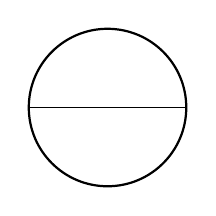
\begin{tikzpicture}\draw[thick] (0,0) circle (1); \draw (-1,0)--(1,0);\end{tikzpicture}
\chapter{Chapter 8}\label{ch:8}
\section{Section 8.1}\label{sec:8-1}
See Chapter~\ref{ch:7} and Section~\ref{sec:8-1}.
\lipsum[42-44]
\begin{equation}\label{eq:8-1} \int_0^{1} x^{8}\,dx = \frac{1^{9}}{9}\end{equation}
\section{Section 8.2}\label{sec:8-2}
See Chapter~\ref{ch:7} and Section~\ref{sec:8-2}.
\lipsum[43-45]
\begin{equation}\label{eq:8-2} \int_0^{2} x^{8}\,dx = \frac{2^{9}}{9}\end{equation}
\section{Section 8.3}\label{sec:8-3}
See Chapter~\ref{ch:7} and Section~\ref{sec:8-3}.
\lipsum[44-46]
\begin{equation}\label{eq:8-3} \int_0^{3} x^{8}\,dx = \frac{3^{9}}{9}\end{equation}
\section{Section 8.4}\label{sec:8-4}
See Chapter~\ref{ch:7} and Section~\ref{sec:8-4}.
\lipsum[45-47]
\begin{equation}\label{eq:8-4} \int_0^{4} x^{8}\,dx = \frac{4^{9}}{9}\end{equation}
\section{Section 8.5}\label{sec:8-5}
See Chapter~\ref{ch:7} and Section~\ref{sec:8-5}.
\lipsum[46-48]
\begin{equation}\label{eq:8-5} \int_0^{5} x^{8}\,dx = \frac{5^{9}}{9}\end{equation}
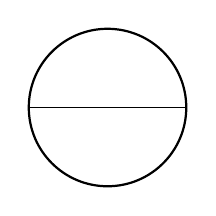
\begin{tikzpicture}\draw[thick] (0,0) circle (1); \draw (-1,0)--(1,0);\end{tikzpicture}
\chapter{Chapter 9}\label{ch:9}
\section{Section 9.1}\label{sec:9-1}
See Chapter~\ref{ch:8} and Section~\ref{sec:9-1}.
\lipsum[47-49]
\begin{equation}\label{eq:9-1} \int_0^{1} x^{9}\,dx = \frac{1^{10}}{10}\end{equation}
\section{Section 9.2}\label{sec:9-2}
See Chapter~\ref{ch:8} and Section~\ref{sec:9-2}.
\lipsum[48-50]
\begin{equation}\label{eq:9-2} \int_0^{2} x^{9}\,dx = \frac{2^{10}}{10}\end{equation}
\section{Section 9.3}\label{sec:9-3}
See Chapter~\ref{ch:8} and Section~\ref{sec:9-3}.
\lipsum[49-51]
\begin{equation}\label{eq:9-3} \int_0^{3} x^{9}\,dx = \frac{3^{10}}{10}\end{equation}
\section{Section 9.4}\label{sec:9-4}
See Chapter~\ref{ch:8} and Section~\ref{sec:9-4}.
\lipsum[50-52]
\begin{equation}\label{eq:9-4} \int_0^{4} x^{9}\,dx = \frac{4^{10}}{10}\end{equation}
\section{Section 9.5}\label{sec:9-5}
See Chapter~\ref{ch:8} and Section~\ref{sec:9-5}.
\lipsum[51-53]
\begin{equation}\label{eq:9-5} \int_0^{5} x^{9}\,dx = \frac{5^{10}}{10}\end{equation}
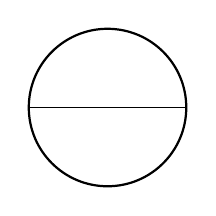
\begin{tikzpicture}\draw[thick] (0,0) circle (1); \draw (-1,0)--(1,0);\end{tikzpicture}
\chapter{Chapter 10}\label{ch:10}
\section{Section 10.1}\label{sec:10-1}
See Chapter~\ref{ch:9} and Section~\ref{sec:10-1}.
\lipsum[52-54]
\begin{equation}\label{eq:10-1} \int_0^{1} x^{10}\,dx = \frac{1^{11}}{11}\end{equation}
\section{Section 10.2}\label{sec:10-2}
See Chapter~\ref{ch:9} and Section~\ref{sec:10-2}.
\lipsum[53-55]
\begin{equation}\label{eq:10-2} \int_0^{2} x^{10}\,dx = \frac{2^{11}}{11}\end{equation}
\section{Section 10.3}\label{sec:10-3}
See Chapter~\ref{ch:9} and Section~\ref{sec:10-3}.
\lipsum[54-56]
\begin{equation}\label{eq:10-3} \int_0^{3} x^{10}\,dx = \frac{3^{11}}{11}\end{equation}
\section{Section 10.4}\label{sec:10-4}
See Chapter~\ref{ch:9} and Section~\ref{sec:10-4}.
\lipsum[55-57]
\begin{equation}\label{eq:10-4} \int_0^{4} x^{10}\,dx = \frac{4^{11}}{11}\end{equation}
\section{Section 10.5}\label{sec:10-5}
See Chapter~\ref{ch:9} and Section~\ref{sec:10-5}.
\lipsum[56-58]
\begin{equation}\label{eq:10-5} \int_0^{5} x^{10}\,dx = \frac{5^{11}}{11}\end{equation}
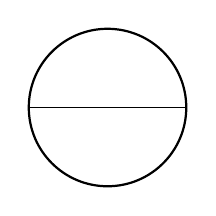
\begin{tikzpicture}\draw[thick] (0,0) circle (1); \draw (-1,0)--(1,0);\end{tikzpicture}
\chapter{Chapter 11}\label{ch:11}
\section{Section 11.1}\label{sec:11-1}
See Chapter~\ref{ch:10} and Section~\ref{sec:11-1}.
\lipsum[57-59]
\begin{equation}\label{eq:11-1} \int_0^{1} x^{11}\,dx = \frac{1^{12}}{12}\end{equation}
\section{Section 11.2}\label{sec:11-2}
See Chapter~\ref{ch:10} and Section~\ref{sec:11-2}.
\lipsum[58-60]
\begin{equation}\label{eq:11-2} \int_0^{2} x^{11}\,dx = \frac{2^{12}}{12}\end{equation}
\section{Section 11.3}\label{sec:11-3}
See Chapter~\ref{ch:10} and Section~\ref{sec:11-3}.
\lipsum[59-61]
\begin{equation}\label{eq:11-3} \int_0^{3} x^{11}\,dx = \frac{3^{12}}{12}\end{equation}
\section{Section 11.4}\label{sec:11-4}
See Chapter~\ref{ch:10} and Section~\ref{sec:11-4}.
\lipsum[60-62]
\begin{equation}\label{eq:11-4} \int_0^{4} x^{11}\,dx = \frac{4^{12}}{12}\end{equation}
\section{Section 11.5}\label{sec:11-5}
See Chapter~\ref{ch:10} and Section~\ref{sec:11-5}.
\lipsum[61-63]
\begin{equation}\label{eq:11-5} \int_0^{5} x^{11}\,dx = \frac{5^{12}}{12}\end{equation}
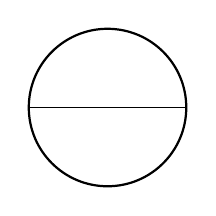
\begin{tikzpicture}\draw[thick] (0,0) circle (1); \draw (-1,0)--(1,0);\end{tikzpicture}
\chapter{Chapter 12}\label{ch:12}
\section{Section 12.1}\label{sec:12-1}
See Chapter~\ref{ch:11} and Section~\ref{sec:12-1}.
\lipsum[62-64]
\begin{equation}\label{eq:12-1} \int_0^{1} x^{12}\,dx = \frac{1^{13}}{13}\end{equation}
\section{Section 12.2}\label{sec:12-2}
See Chapter~\ref{ch:11} and Section~\ref{sec:12-2}.
\lipsum[63-65]
\begin{equation}\label{eq:12-2} \int_0^{2} x^{12}\,dx = \frac{2^{13}}{13}\end{equation}
\section{Section 12.3}\label{sec:12-3}
See Chapter~\ref{ch:11} and Section~\ref{sec:12-3}.
\lipsum[64-66]
\begin{equation}\label{eq:12-3} \int_0^{3} x^{12}\,dx = \frac{3^{13}}{13}\end{equation}
\section{Section 12.4}\label{sec:12-4}
See Chapter~\ref{ch:11} and Section~\ref{sec:12-4}.
\lipsum[65-67]
\begin{equation}\label{eq:12-4} \int_0^{4} x^{12}\,dx = \frac{4^{13}}{13}\end{equation}
\section{Section 12.5}\label{sec:12-5}
See Chapter~\ref{ch:11} and Section~\ref{sec:12-5}.
\lipsum[66-68]
\begin{equation}\label{eq:12-5} \int_0^{5} x^{12}\,dx = \frac{5^{13}}{13}\end{equation}
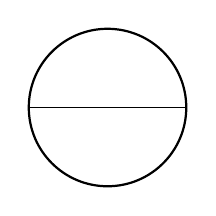
\begin{tikzpicture}\draw[thick] (0,0) circle (1); \draw (-1,0)--(1,0);\end{tikzpicture}
\end{document}
